
\documentclass[12pt,hyperref,a4paper,UTF8,twoside]{ctexart}
\usepackage{XTUReport}
\usepackage{amsmath,amssymb,amsfonts,amsthm,bm,mathtools}
\usepackage{geometry}
\usepackage{graphicx}
\usepackage{booktabs}
\usepackage{float}
\usepackage{caption}
\usepackage{subcaption}
\usepackage{enumitem}
\usepackage{hyperref}
\usepackage{setspace}
\usepackage{array}
\usepackage{siunitx}
\usepackage{xcolor}
\usepackage{longtable}

\geometry{left=2.6cm,right=2.6cm,top=2.6cm,bottom=2.6cm}
\onehalfspacing
\setlength{\parindent}{2em}
\setlength{\parskip}{0.12em}
\captionsetup{font=small,labelfont=bf}
\hypersetup{colorlinks=true,linkcolor=blue,citecolor=blue,urlcolor=blue}

\newtheorem{definition}{定义}
\newtheorem{proposition}{命题}
\newtheorem{remark}{注}
\newcommand{\dd}{\mathrm d}
\newcommand{\R}{\mathbb R}
\newcommand{\e}{\mathrm e}
\newcommand{\ii}{\mathrm i}
\newcommand{\calF}{\mathcal F}
\newcommand{\calL}{\mathcal L}
\newcommand{\calJ}{\mathcal J}
\newcommand{\norm}[1]{\left\lVert #1\right\rVert}
\newcommand{\ip}[2]{\left\langle #1,#2\right\rangle}
\DeclareMathOperator*{\argmin}{arg\,min}

\setlength{\headheight}{15pt}
\begin{document}
\cover%封面
\thispagestyle{empty}
%中文摘要
\newpage
\pagestyle{abstractcnstyle}
\pagenumbering{Roman}
\begin{abstractcn}
神经网络方法近年来被广泛用于偏微分方程的数值求解,其中物理信息神经网络(Physics-Informed Neural Networks, PINN)通过把微分方程残差与边界条件写入损失函数,为无网格求解 PDE 提供了一种灵活框架。然而,神经网络的表达能力并不等同于训练过程的有效可达性。已有研究表明,标准多层感知机在梯度型训练中通常具有明显的谱偏差:低频成分较早被拟合,而高频成分收敛较慢。Helmholtz 方程是典型的振荡型方程,高波数情形下解的主频率与波数 $k$ 同阶,因此普通 MLP 或强形式 PINN 在求解时会面临训练困难、相位误差、采样不足与残差尺度放大等问题。本文从 Fourier 分解、线性化训练动力学和 Helmholtz 算子符号三个角度分析谱偏差的数学机制,建立误差频率与残差放大的关系,并通过一维函数拟合和一维 Helmholtz-PINN 实验展示低频目标与高频目标之间的训练差异。实验表明:普通 MLP 对低频函数拟合较快,而对高频函数误差下降明显变慢；在 Helmholtz-PINN 中,波数增大时相对误差和残差显著恶化。Fourier features 能改善高频函数的表示能力,但强形式 PINN 仍受到优化、采样和残差尺度的制约。本文最后讨论了波数相关特征、损失归一化、自适应采样和弱形式 PINN 等改进方向。
\end{abstractcn}

\keywordscn{神经网络；谱偏差；频率原则；Helmholtz 方程；PINN；Fourier features}

\newpage
\pagestyle{contentstyle}
\tableofcontents

\newpage
\pagestyle{articlestyle} % 切换回正文页眉样式
\pagenumbering{arabic} % 设置页码样式为阿拉伯数字
\setcounter{page}{1}   % 正文页码从1开始


\section{引言}

深度神经网络在机器学习中具有强大的函数表示能力。与传统数值方法相比,神经网络求解偏微分方程(partial differential equations, PDEs)的一个突出特点是:它不必先构造固定网格上的离散函数空间,而是直接用带参数的函数族表示未知解。设 PDE 的未知解为 $u$,神经网络方法通常构造
\begin{equation}\label{eq:basic-approx}
    u(x)\approx u_\theta(x),
\end{equation}
其中 $\theta$ 表示网络权重和偏置。训练过程就是通过最小化损失函数确定 $\theta$。若损失函数中包含 PDE 残差、边界条件残差和可能的观测数据残差,就得到物理信息神经网络(Physics-Informed Neural Networks, PINN)的基本框架\cite{raissi2019physics}。

PINN 的形式非常自然；它也可以看作 Deep Galerkin Method 等无网格 PDE 学习方法的一种代表性实现\cite{sirignano2018dgm,lu2021deepxde,karniadakis2021physics}. 考虑边值问题
\begin{equation}\label{eq:pde-general}
    \calL u=f\quad \text{in }\Omega,\qquad
    \mathcal B u=g\quad \text{on }\partial\Omega,
\end{equation}
其中 $\calL$ 是微分算子,$\mathcal B$ 是边界算子。令 $u_\theta$ 为神经网络近似解,PINN 通常最小化如下经验损失:
\begin{equation}\label{eq:pinn-loss-general}
\begin{aligned}
    \calJ(\theta)
    &=\calJ_r(\theta)+\lambda\calJ_b(\theta),\\
    \calJ_r(\theta)
    &=\frac{1}{N_r}\sum_{i=1}^{N_r}
    \left|\calL u_\theta(x_i)-f(x_i)\right|^2,\\
    \calJ_b(\theta)
    &=\frac{1}{N_b}\sum_{j=1}^{N_b}
    \left|\mathcal B u_\theta(y_j)-g(y_j)\right|^2.
\end{aligned}
\end{equation}
这里 $x_i$ 是区域内部采样点,$y_j$ 是边界采样点,$\lambda$ 是用于平衡边界项与内部残差项的权重。由于自动微分可以计算 $u_\theta$ 的导数,PINN 在形式上可以处理多种微分方程和边界条件。

不过,神经网络的“可表达”与“可训练”是两个不同问题。万能逼近定理说明,在一定条件下,神经网络可以逼近广泛的连续函数\cite{cybenko1989approximation,hornik1989multilayer}；但这并不说明实际优化过程一定可以高效地找到相应参数。Rahaman 等\cite{rahaman2019spectral}和 Xu 等\cite{xu2020frequency}从 Fourier 角度指出,标准深度网络训练中常表现出低频优先的现象,即网络倾向于先拟合目标函数的低频成分,再逐渐拟合高频成分。这种现象通常被称为谱偏差(spectral bias)或频率原则(frequency principle)。

谱偏差对 Helmholtz 方程尤其重要。Helmholtz 方程的一般形式为
\begin{equation}\label{eq:helmholtz-general}
    -\Delta u-k^2u=f,
\end{equation}
其中 $k>0$ 是波数。该方程描述固定频率下的波动问题,其解通常具有明显振荡性。当 $k$ 增大时,波长缩短,解在同一区域内振荡次数增加。对于传统有限元方法,高波数 Helmholtz 问题会带来网格分辨率要求、相位误差和污染效应等困难\cite{ihlenburg1998finite,babuska1997pollution,melenk2011wavenumber,ernst2012helmholtz}。对于 PINN,除这些波动问题本身的困难外,还叠加了神经网络低频优先训练的谱偏差。因此,研究谱偏差对 Helmholtz 方程求解的影响,不仅有助于理解 PINN 的局限,也有助于认识机器学习方法在科学计算中的适用边界。

本文围绕以下问题展开:
\begin{enumerate}[label=(\arabic*)]
    \item 神经网络训练中的低频优先现象如何用 Fourier 分解和训练动力学表达？
    \item Helmholtz 算子的频率符号如何放大相位误差和频率误差？
    \item Fourier features 为什么能缓解高频函数拟合,却不一定完全解决强形式 PINN 的困难？
\end{enumerate}
全文结构如下:第 2 节介绍神经网络函数逼近与谱偏差；第 3 节给出 PINN 的误差来源；第 4 节分析 Helmholtz 方程的振荡结构与频域符号；第 5 节讨论谱偏差对 Helmholtz-PINN 的具体影响；第 6 节给出可复现实验；第 7 节讨论可能改进；第 8 节总结全文。

\section{神经网络函数逼近与谱偏差}

\subsection{多层感知机作为参数化函数族}

考虑标准前馈神经网络。给定输入 $x\in\R^d$,一个 $L$ 层多层感知机(multi-layer perceptron, MLP)可以写为
\begin{equation}\label{eq:mlp}
\begin{aligned}
    h_0(x)&=x,\\
    h_\ell(x)&=\sigma(W_\ell h_{\ell-1}(x)+b_\ell),\qquad \ell=1,\dots,L-1,\\
    u_\theta(x)&=W_Lh_{L-1}(x)+b_L.
\end{aligned}
\end{equation}
其中 $W_\ell,b_\ell$ 为可训练参数,$\sigma$ 是非线性激活函数,例如 $\tanh$ 或 ReLU。监督训练通常最小化经验风险
\begin{equation}\label{eq:empirical-risk}
    \min_\theta \frac1N\sum_{i=1}^N |u_\theta(x_i)-f(x_i)|^2.
\end{equation}
从函数逼近角度看,网络 $u_\theta$ 给出了一个非线性参数化函数族。它与多项式、三角函数、有限元基函数等传统近似空间不同:网络参数并不是线性系数,优化问题通常也是非凸的。

虽然深度网络表达能力很强,但训练过程受到优化算法、初始化、激活函数光滑性和损失函数结构的影响。特别是,当目标函数具有复杂的高频结构时,即使网络宽度和深度足够,优化过程也未必能快速学习这些高频成分。

\subsection{Fourier 视角下的误差分解}

为清楚表达“频率”概念,先考虑周期区间 $[0,2\pi]$ 上的函数。若
\begin{equation}\label{eq:fourier-series}
    f(x)=\sum_{m\in\mathbb Z}\widehat f_m\e^{\ii mx},
    \qquad
    \widehat f_m=\frac1{2\pi}\int_0^{2\pi} f(x)\e^{-\ii mx}\,\dd x,
\end{equation}
则 Parseval 恒等式给出
\begin{equation}\label{eq:parseval}
    \norm{f}_{L^2(0,2\pi)}^2=2\pi\sum_{m\in\mathbb Z}|\widehat f_m|^2.
\end{equation}
令 $e_\theta=u_\theta-f$,其频率误差为
\begin{equation}\label{eq:fourier-error}
    \widehat e_m(\theta)=\widehat{u_\theta}_m-\widehat f_m.
\end{equation}
于是总的 $L^2$ 误差可分解为不同频率误差之和:
\begin{equation}\label{eq:l2-frequency-decomposition}
    \norm{u_\theta-f}_{L^2}^2
    =2\pi\sum_{m\in\mathbb Z}|\widehat e_m(\theta)|^2.
\end{equation}

\begin{definition}[谱偏差]
若在梯度型训练过程中,低频系数 $|\widehat e_m(t)|$ 通常比高频系数更快衰减,即对较小 $|m|$ 的模式有更快的误差下降,而对较大 $|m|$ 的模式误差下降较慢,则称该训练过程具有谱偏差或低频优先现象。
\end{definition}

例如,考虑
\begin{equation}\label{eq:sin-example}
    f_1(x)=\sin(5x),\qquad f_2(x)=\sin(40x),\quad x\in[0,1].
\end{equation}
两个函数的解析表达式都很简单,但 $f_2$ 在区间上的振荡次数明显更多。普通 MLP 在相同训练预算下通常更容易拟合 $f_1$,而对 $f_2$ 的误差下降较慢。这说明神经网络训练难度不仅取决于函数公式是否简单,也取决于目标函数的频率结构。

\subsection{线性化训练动力学解释}

谱偏差还可以从线性化训练动力学理解。考虑平方损失
\begin{equation}\label{eq:square-loss-cont}
    \calJ(\theta)=\frac12\int_\Omega |u_\theta(x)-f(x)|^2\,\dd x.
\end{equation}
这一视角与 NTK 理论有关,Jacot 等证明了无限宽极限下网络训练可由核梯度流描述\cite{jacot2018neural}。若在初始化 $\theta_0$ 附近线性化网络:
\begin{equation}\label{eq:linearization}
    u_\theta(x)\approx u_{\theta_0}(x)+\nabla_\theta u_{\theta_0}(x)\cdot(\theta-\theta_0),
\end{equation}
则梯度流近似满足
\begin{equation}\label{eq:ntk-flow}
    \partial_t u_t(x)=-\int_\Omega K_{\theta_0}(x,y)\bigl(u_t(y)-f(y)\bigr)\,\dd y,
\end{equation}
其中
\begin{equation}\label{eq:ntk-kernel}
    K_{\theta_0}(x,y)=\nabla_\theta u_{\theta_0}(x)\cdot \nabla_\theta u_{\theta_0}(y)
\end{equation}
是神经切线核(neural tangent kernel, NTK)。若积分算子 $K$ 有特征分解
\begin{equation}\label{eq:kernel-eigendecomp}
    K\phi_j=\lambda_j\phi_j,
\end{equation}
并将误差写为
\begin{equation}\label{eq:error-mode}
    e_t(x)=u_t(x)-f(x)=\sum_j c_j(t)\phi_j(x),
\end{equation}
则由式\eqref{eq:ntk-flow}得到
\begin{equation}\label{eq:mode-decay}
    \frac{\dd}{\dd t}c_j(t)=-\lambda_jc_j(t),
    \qquad
    c_j(t)=c_j(0)\e^{-\lambda_jt}.
\end{equation}
因此,误差模式的收敛速度由特征值 $\lambda_j$ 决定。若高频模式对应较小的 $\lambda_j$,则高频误差衰减慢,表现为低频优先。这一推导不是对所有网络的完整证明,但它给出了谱偏差的一个清晰数学图像:训练不是均匀地压低所有频率,而是由网络结构和优化动力学决定不同模式的衰减速度。

\subsection{Fourier features 的基本思想}

为了缓解普通 MLP 对高频函数学习困难的问题,Tancik 等\cite{tancik2020fourier}提出并系统研究了 Fourier feature mapping。其核心思想是先把低维坐标 $x$ 映射为含有三角函数的高维特征:
\begin{equation}\label{eq:fourier-feature}
    \gamma(x)=\bigl(\sin(Bx),\cos(Bx)\bigr),
\end{equation}
再用 MLP 学习
\begin{equation}\label{eq:fourier-network}
    u_\theta(x)=N_\theta(\gamma(x)).
\end{equation}
若一维情形下选择频率集合 $\{\omega_j\}_{j=1}^M$,则可以写成
\begin{equation}\label{eq:feature-vector-1d}
    \gamma(x)=\bigl(\sin(\omega_1x),\cos(\omega_1x),\dots,
    \sin(\omega_Mx),\cos(\omega_Mx)\bigr).
\end{equation}
Fourier features 的意义在于:高频振荡不再完全由网络隐层从原始坐标中“慢慢学出”。与此相关,使用周期激活函数的 SIREN 也被用于表示高频信号及其导数\cite{sitzmann2020implicit}。因此,高频信息可以通过输入特征或网络结构被显式编码。,而是在输入层就被显式提供。对于含有已知波数 $k$ 的 Helmholtz 方程,这一思想尤其自然,因为解的主要振荡频率往往与 $k$ 相关。

\section{PINN 的误差来源与数学结构}

\subsection{强形式残差与经验积分}

设精确解满足式\eqref{eq:pde-general}。PINN 的理想连续损失可写为
\begin{equation}\label{eq:continuous-pinn-loss}
    \calJ_{\mathrm{cont}}(\theta)
    =\norm{\calL u_\theta-f}_{L^2(\Omega)}^2
    +\lambda\norm{\mathcal B u_\theta-g}_{L^2(\partial\Omega)}^2.
\end{equation}
实际训练中使用采样点近似积分:
\begin{equation}\label{eq:quadrature-loss}
    \calJ_{N}(\theta)
    =\frac1{N_r}\sum_{i=1}^{N_r}|\calL u_\theta(x_i)-f(x_i)|^2
    +\lambda\frac1{N_b}\sum_{j=1}^{N_b}|\mathcal B u_\theta(y_j)-g(y_j)|^2.
\end{equation}
PINN 的训练还会受到复合损失项梯度尺度不平衡的影响,这一点在 Wang 等关于 PINN 梯度病态的研究中有系统讨论\cite{wang2021understanding}。因此误差来源至少包括三类:
\begin{equation}\label{eq:error-decomp-informal}
    E_{\mathrm{total}}
    \approx
    E_{\mathrm{app}}+E_{\mathrm{opt}}+E_{\mathrm{sample}}.
\end{equation}
更具体地,若 $\Theta$ 是网络参数集合,则可以形式地写成
\begin{equation}\label{eq:error-components}
\begin{aligned}
    \underbrace{\norm{u-u_{\theta_T}}}_{\text{total}}
    \leq{}&
    \underbrace{\inf_{\theta\in\Theta}\norm{u-u_\theta}}_{\text{approximation}}
    +\underbrace{\norm{u_{\theta_*}-u_{\theta_T}}}_{\text{optimization}}\\
    &+\underbrace{\bigl|\calJ_{\mathrm{cont}}(\theta)-\calJ_N(\theta)\bigr|}_{\text{sampling}},
\end{aligned}
\end{equation}
其中 $\theta_T$ 表示训练 $T$ 步后的参数,$\theta_*$ 表示理想损失下的最优参数。式\eqref{eq:error-components}不是严格定理,而是用于说明 PINN 与传统离散方法的差异:即使表达空间足够大,优化和采样仍可能成为主要瓶颈。

\subsection{强形式与弱形式的比较}

有限元方法通常先构造有限维空间 $V_h$,再寻找 $u_h\in V_h$ 使得
\begin{equation}\label{eq:fem-weak}
    a(u_h,v_h)=F(v_h),\quad \forall v_h\in V_h.
\end{equation}
这里的弱形式、测试函数和试探函数空间都具有明确的变分意义。以一维 Poisson 方程为例:
\begin{equation}\label{eq:poisson-model}
    -u''=f,\quad u(0)=u(1)=0.
\end{equation}
乘以测试函数 $v\in H_0^1(0,1)$ 并分部积分,有
\begin{equation}\label{eq:poisson-weak}
    \int_0^1 u'(x)v'(x)\,\dd x=\int_0^1 f(x)v(x)\,\dd x.
\end{equation}
相比之下,强形式 PINN 直接最小化
\begin{equation}\label{eq:poisson-strong-loss}
    \int_0^1|-u_\theta''(x)-f(x)|^2\,\dd x,
\end{equation}
这要求网络二阶导数足够准确。对于 Helmholtz 方程,这个问题更加明显,因为强形式残差包含二阶导数项和 $k^2u$ 项之间的精确抵消。

\section{Helmholtz 方程的振荡结构与频域符号}

\subsection{一维模型问题与非共振条件}

为突出主要机制,本文考虑一维 Helmholtz 方程:
\begin{equation}\label{eq:helmholtz-1d}
    -u''(x)-k^2u(x)=f(x),\quad x\in(0,1).
\end{equation}
齐次方程
\begin{equation}\label{eq:homogeneous-eq}
    -u''-k^2u=0
\end{equation}
的通解为
\begin{equation}\label{eq:homogeneous-solution}
    u(x)=A\cos(kx)+B\sin(kx).
\end{equation}
因此,$k$ 直接决定了解的振荡频率。$k$ 越大,波长
\begin{equation}\label{eq:wavelength}
    \lambda_{\mathrm{wave}}=\frac{2\pi}{k}
\end{equation}
越短,单位区间内振荡次数越多。

考虑 Dirichlet 边界条件 $u(0)=u(1)=0$。若 $k=n\pi$,则 $\sin(kx)=\sin(n\pi x)$ 是非零齐次解,问题不唯一。因此 Dirichlet Helmholtz 问题的非共振条件是
\begin{equation}\label{eq:nonresonance}
    k\notin \pi\mathbb N.
\end{equation}
本文实验选择 $k=5,10,20,40$,这些数值均不等于 $n\pi$,从而避免特征值导致的非唯一性。

实验中使用制造解
\begin{equation}\label{eq:manufactured-solution}
    u(x)=\sin(kx),
\end{equation}
并取 $f(x)=0$,因为
\begin{equation}\label{eq:manufactured-check}
    -u''(x)-k^2u(x)=k^2\sin(kx)-k^2\sin(kx)=0.
\end{equation}
边界条件取
\begin{equation}\label{eq:dirichlet-bc}
    u(0)=0,
    \qquad
    u(1)=\sin k.
\end{equation}

\subsection{Helmholtz 算子的 Fourier 符号}

在全空间或周期区间中,考虑 Fourier 模式
\begin{equation}\label{eq:fourier-mode}
    \phi_\xi(x)=\e^{\ii \xi x}.
\end{equation}
一维 Helmholtz 算子
\begin{equation}\label{eq:helmholtz-operator}
    \calL_k=-\frac{\dd^2}{\dd x^2}-k^2
\end{equation}
作用在 $\phi_\xi$ 上得到
\begin{equation}\label{eq:symbol}
    \calL_k\phi_\xi
    =\left(\xi^2-k^2\right)\phi_\xi.
\end{equation}
因此 Helmholtz 算子的 Fourier 符号为
\begin{equation}\label{eq:helmholtz-symbol}
    p_k(\xi)=\xi^2-k^2.
\end{equation}
这说明 Helmholtz 方程的特征频率位于 $|\xi|=k$ 附近。若网络主要学习到低频 $|\xi|\ll k$,则
\begin{equation}\label{eq:low-frequency-symbol}
    |p_k(\xi)|=|\xi^2-k^2|\approx k^2,
\end{equation}
残差不会小。只有当网络近似中包含接近 $\xi=\pm k$ 的振荡模式时,才可能有效降低残差。

\begin{proposition}[单频误差的残差放大]\label{prop:residual-amplification}
设误差 $e(x)=A\sin(qx)$。则 Helmholtz 残差误差为
\begin{equation}\label{eq:residual-single-frequency}
    \calL_k e=(q^2-k^2)A\sin(qx).
\end{equation}
因此
\begin{equation}\label{eq:residual-error-norm}
    \norm{\calL_k e}_{L^2(0,1)}
    =|q^2-k^2|\,\norm{e}_{L^2(0,1)}.
\end{equation}
特别地,若 $q=k+\delta$,则
\begin{equation}\label{eq:phase-frequency-error}
    q^2-k^2=2k\delta+\delta^2.
\end{equation}
当 $k$ 较大时,即使频率偏差 $\delta$ 很小,残差也可能被 $2k\delta$ 放大。
\end{proposition}

命题\ref{prop:residual-amplification}揭示了 Helmholtz-PINN 的核心困难:强形式残差不只要求函数值接近,还要求网络学到正确的振荡频率和相位。若网络由于谱偏差长期停留在低频近似上,则残差很难真正下降。

\subsection{变分形式与非强制性}

对 Dirichlet 问题,将式\eqref{eq:helmholtz-1d}乘以测试函数 $v\in H_0^1(0,1)$ 并分部积分,得到弱形式:求 $u\in H_0^1(0,1)$ 使
\begin{equation}\label{eq:helmholtz-weak}
    a_k(u,v)=F(v),\qquad \forall v\in H_0^1(0,1),
\end{equation}
其中
\begin{equation}\label{eq:helmholtz-bilinear}
    a_k(u,v)=\int_0^1 u'(x)v'(x)\,\dd x-k^2\int_0^1u(x)v(x)\,\dd x,
\end{equation}
\begin{equation}\label{eq:right-hand-functional}
    F(v)=\int_0^1 f(x)v(x)\,\dd x.
\end{equation}
与 Poisson 方程不同,
\begin{equation}\label{eq:not-coercive}
    a_k(v,v)=\norm{v'}_{L^2}^2-k^2\norm{v}_{L^2}^2
\end{equation}
不一定为正,因此无法直接得到 Poisson 型强制性估计。不过它满足 G\aa rding 型结构:
\begin{equation}\label{eq:garding}
    a_k(v,v)+k^2\norm{v}_{L^2}^2=\norm{v'}_{L^2}^2.
\end{equation}
这说明 Helmholtz 方程具有“椭圆主部 + 不定零阶项”的结构,分析和数值稳定性都比 Poisson 方程更微妙。

\section{谱偏差对 Helmholtz-PINN 的影响}

\subsection{强形式残差中的敏感抵消}

对一维 Helmholtz 方程,PINN 残差为
\begin{equation}\label{eq:helmholtz-residual}
    r_\theta(x)=-u_\theta''(x)-k^2u_\theta(x)-f(x).
\end{equation}
当 $f=0$ 且精确解为 $\sin(kx)$ 时,精确解满足
\begin{equation}\label{eq:sensitive-cancel}
    -u''=k^2u.
\end{equation}
这意味着方程要求二阶导数项与零阶项之间发生精确抵消。若网络近似在相位上稍有偏差,$u_\theta''$ 与 $k^2u_\theta$ 的抵消就会被破坏,残差可能显著增大。

为了说明相位误差的影响,设网络学到的函数近似为
\begin{equation}\label{eq:wrong-phase}
    u_\theta(x)=\sin(kx+\varphi).
\end{equation}
若边界条件暂不考虑,则它仍满足齐次 Helmholtz 方程,因为频率仍为 $k$。但是边界条件会出现误差:
\begin{equation}\label{eq:phase-boundary-error}
    u_\theta(0)-u(0)=\sin\varphi,
    \qquad
    u_\theta(1)-u(1)=\sin(k+\varphi)-\sin k.
\end{equation}
若频率也有偏差,即
\begin{equation}\label{eq:wrong-frequency}
    u_\theta(x)=\sin((k+\delta)x),
\end{equation}
则由命题\ref{prop:residual-amplification}有
\begin{equation}\label{eq:wrong-frequency-residual}
    \calL_k u_\theta=((k+\delta)^2-k^2)\sin((k+\delta)x)
    =(2k\delta+\delta^2)\sin((k+\delta)x).
\end{equation}
这说明高波数情形下的频率误差会被 $k$ 放大。

\subsection{采样分辨率与波长}

PINN 损失是在有限采样点上计算的。对于高频解,如果内部采样点数量不足,训练过程可能只在采样点处降低残差,而无法保证采样点之间的行为正确。设波长为 $\lambda_{\mathrm{wave}}=2\pi/k$。若使用均匀采样点间距 $h_s$,则每个波长上的采样点数大约为
\begin{equation}\label{eq:points-per-wavelength}
    N_{\lambda}\approx \frac{\lambda_{\mathrm{wave}}}{h_s}=\frac{2\pi}{kh_s}.
\end{equation}
为了观察振荡结构,至少需要 $N_\lambda$ 不太小。若 $kh_s$ 较大,则损失函数本身就无法充分分辨振荡。这个现象与传统网格方法中的“每个波长需要若干自由度”相似,但在 PINN 中还叠加了优化偏差。

\subsection{损失尺度随波数放大}

强形式残差中有 $k^2u_\theta$ 项。因此在不同 $k$ 的问题之间直接比较残差 MSE 并不公平。若令
\begin{equation}\label{eq:normalized-residual}
    \widetilde r_\theta(x)=\frac{-u_\theta''(x)-k^2u_\theta(x)-f(x)}{1+k^2},
\end{equation}
则归一化残差可以减弱 $k$ 增大造成的尺度变化。在实际训练中,若不做类似归一化,优化器可能面对随 $k$ 急剧变大的梯度尺度,导致训练不稳定。

进一步设误差 $e=u_\theta-u$,且边界条件被硬约束满足。由于 $\calL_k u=f$,有
\begin{equation}\label{eq:residual-equals-error}
    r_\theta=\calL_k u_\theta-f=\calL_k e.
\end{equation}
在频域中,若
\begin{equation}\label{eq:error-fourier}
    e(x)=\sum_\xi \widehat e(\xi)\e^{\ii\xi x},
\end{equation}
则
\begin{equation}\label{eq:residual-fourier}
    \widehat r(\xi)=(\xi^2-k^2)\widehat e(\xi),
\end{equation}
于是
\begin{equation}\label{eq:residual-fourier-norm}
    \norm{r}_{L^2}^2
    \sim\sum_\xi |\xi^2-k^2|^2 |\widehat e(\xi)|^2.
\end{equation}
式\eqref{eq:residual-fourier-norm}清楚表明:Helmholtz 残差对频率结构十分敏感。PINN 不是简单拟合 $u$,而是在频域上用权重 $|\xi^2-k^2|^2$ 惩罚误差。

\section{数值实验}

本节给出两个实验。实验代码使用 Python 与 PyTorch 实现,所有图表均由随文代码生成。为了保证实验可重复,代码中固定随机种子为 20260608。实验目的不是追求最优 PINN 调参,而是在统一训练预算下展示低频目标与高频目标之间的差异。

\subsection{实验一:函数拟合中的谱偏差}

考虑区间 $[0,1]$ 上的函数拟合问题:
\begin{equation}\label{eq:fit-functions}
    f_k(x)=\sin(kx),\qquad k=5,40.
\end{equation}
普通 MLP 直接输入 $x$,Fourier-MLP 先使用
\begin{equation}\label{eq:experiment-features}
    \gamma_k(x)=\bigl(\sin(\omega_jx),\cos(\omega_jx)\bigr)_{j=1}^M,
    \qquad
    \{\omega_j\}=\{1,2,4,8,16,32,k\}
\end{equation}
进行特征映射。训练损失为均方误差:
\begin{equation}\label{eq:mse-fit}
    \calJ_{\mathrm{fit}}(\theta)=\frac1N\sum_{i=1}^N |u_\theta(x_i)-\sin(kx_i)|^2.
\end{equation}
测试误差使用相对 $L^2$ 误差:
\begin{equation}\label{eq:relative-l2}
    E_{L^2}=\frac{\norm{u_\theta-u}_{L^2(0,1)}}{\norm{u}_{L^2(0,1)}}.
\end{equation}

图\ref{fig:spectral-training}展示了相对 $L^2$ 误差随训练轮数的变化。普通 MLP 对 $k=5$ 的低频目标拟合较快,但对 $k=40$ 的高频目标误差下降缓慢；Fourier-MLP 由于显式引入三角特征,对高频函数拟合明显更好。这与谱偏差理论一致:普通网络倾向于低频优先,而 Fourier features 可以改善低维高频函数表示。

\begin{figure}[H]
    \centering
    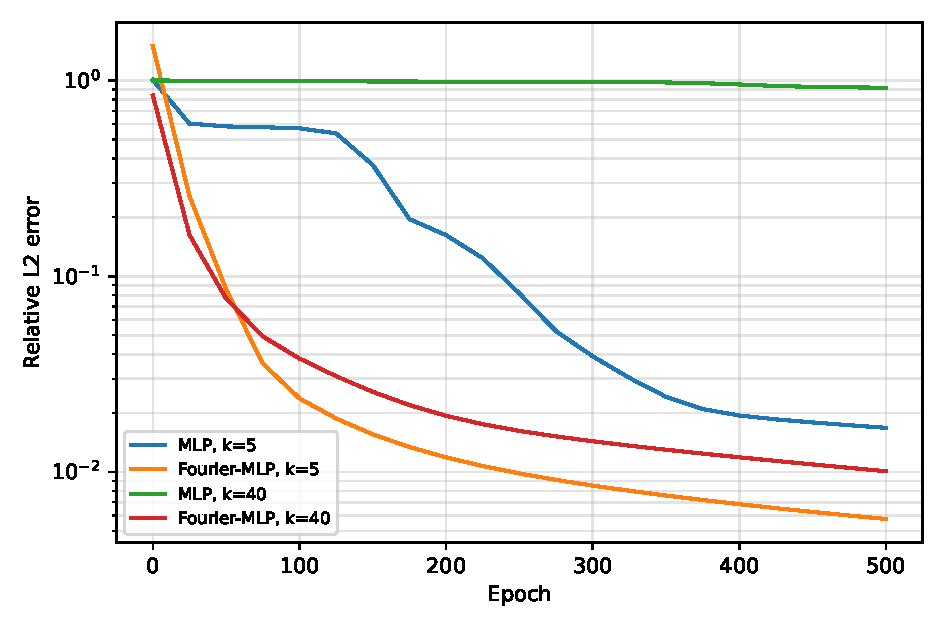
\includegraphics[width=0.78\textwidth]{figures/fig_spectral_bias_training.pdf}
    \caption{函数拟合实验中的相对 $L^2$ 误差。普通 MLP 对低频目标收敛较快,对高频目标收敛明显变慢；Fourier-MLP 在高频目标上表现更好。}
    \label{fig:spectral-training}
\end{figure}

图\ref{fig:fit-comparison}进一步展示了最终拟合曲线。对低频函数,两种模型都能给出较好近似；对高频函数,普通 MLP 在相同训练预算下无法捕捉完整振荡,而 Fourier-MLP 明显更接近精确函数。

\begin{figure}[H]
    \centering
    \subfigure[$\sin(5x)$]{
        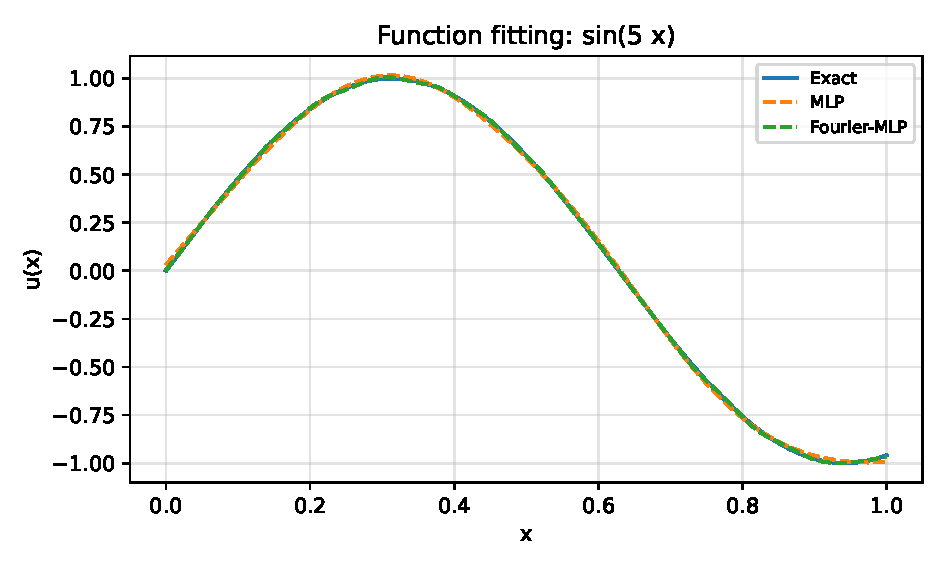
\includegraphics[width=0.48\textwidth]{figures/fig_fit_k5.pdf}
    }
    \hfill
    \subfigure[$\sin(40x)$]{
        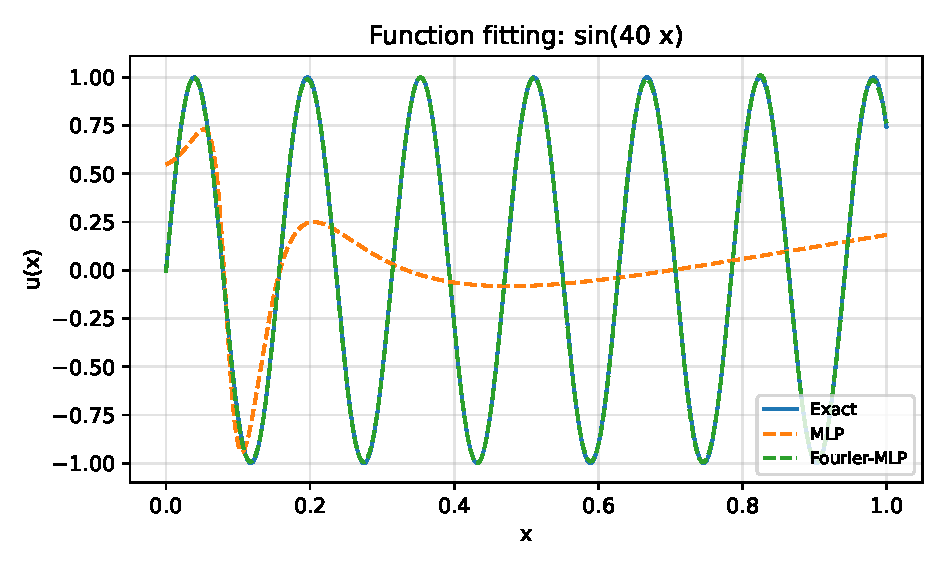
\includegraphics[width=0.48\textwidth]{figures/fig_fit_k40.pdf}
    }
    \caption{低频与高频函数的拟合结果。}
    \label{fig:fit-comparison}
\end{figure}

\subsection{实验二:一维 Helmholtz 方程的 PINN 求解}

考虑齐次 Helmholtz 方程
\begin{equation}\label{eq:experiment-helmholtz}
    -u''(x)-k^2u(x)=0,
    \qquad x\in(0,1),
\end{equation}
边界条件为
\begin{equation}\label{eq:experiment-bc}
    u(0)=0,
    \qquad
    u(1)=\sin k,
\end{equation}
精确解为 $u(x)=\sin(kx)$。为了严格满足边界条件,本文采用硬约束试探函数
\begin{equation}\label{eq:hard-constraint}
    u_\theta(x)=x\sin k+x(1-x)N_\theta(x),
\end{equation}
其中 $N_\theta$ 是神经网络。因为
\begin{equation}\label{eq:hard-bc-check}
    u_\theta(0)=0,
    \qquad
    u_\theta(1)=\sin k,
\end{equation}
边界条件自动满足,训练时只需要最小化内部残差
\begin{equation}\label{eq:pinn-residual-loss}
    \calJ_r(\theta)=\frac1{N_r}\sum_{i=1}^{N_r}
    \left|-u_\theta''(x_i)-k^2u_\theta(x_i)\right|^2.
\end{equation}

表\ref{tab:pinn-results}给出了不同波数下普通 MLP-PINN 与 Fourier-PINN 的最终残差均方误差和相对 $L^2$ 误差。随着 $k$ 从 5 增大到 40,普通 MLP-PINN 的误差明显恶化。Fourier 特征在较高波数下能降低部分残差,但相对 $L^2$ 误差仍接近 1,说明仅改善输入特征不能自动解决强形式 Helmholtz-PINN 的训练问题。这里的实验结果应理解为对困难机制的展示,而不是对各种 PINN 技巧调参后的最优性能比较。

\begin{table}[H]
\centering
\caption{一维 Helmholtz-PINN 实验结果。Rel-$L^2$ 表示相对 $L^2(0,1)$ 误差。}
\label{tab:pinn-results}
\begin{tabular}{cccc}
\toprule
波数 $k$ & 模型 & 最终残差 MSE & Rel-$L^2$ 误差 \\
\midrule
5  & MLP-PINN     & $1.4160$             & $2.2000\times 10^{-2}$ \\
5  & Fourier-PINN & $1.0280\times 10^{2}$& $8.2887\times 10^{-1}$ \\
10 & MLP-PINN     & $3.5622\times 10^{2}$& $1.0773$ \\
10 & Fourier-PINN & $5.8248\times 10^{1}$& $9.5397\times 10^{-1}$ \\
20 & MLP-PINN     & $1.1746\times 10^{4}$& $1.0660$ \\
20 & Fourier-PINN & $4.2071\times 10^{3}$& $9.8514\times 10^{-1}$ \\
40 & MLP-PINN     & $1.1326\times 10^{5}$& $1.0087$ \\
40 & Fourier-PINN & $8.1840\times 10^{4}$& $9.6754\times 10^{-1}$ \\
\bottomrule
\end{tabular}
\end{table}

图\ref{fig:pinn-training}展示了部分波数下相对误差的训练曲线。可以看出,$k=5$ 时普通 MLP-PINN 能较快达到较小误差,而 $k=20,40$ 时误差长期停留在较高水平。这与前文的分析一致:波数越大,解的高频结构越明显,谱偏差和残差尺度问题越突出。

\begin{figure}[H]
    \centering
    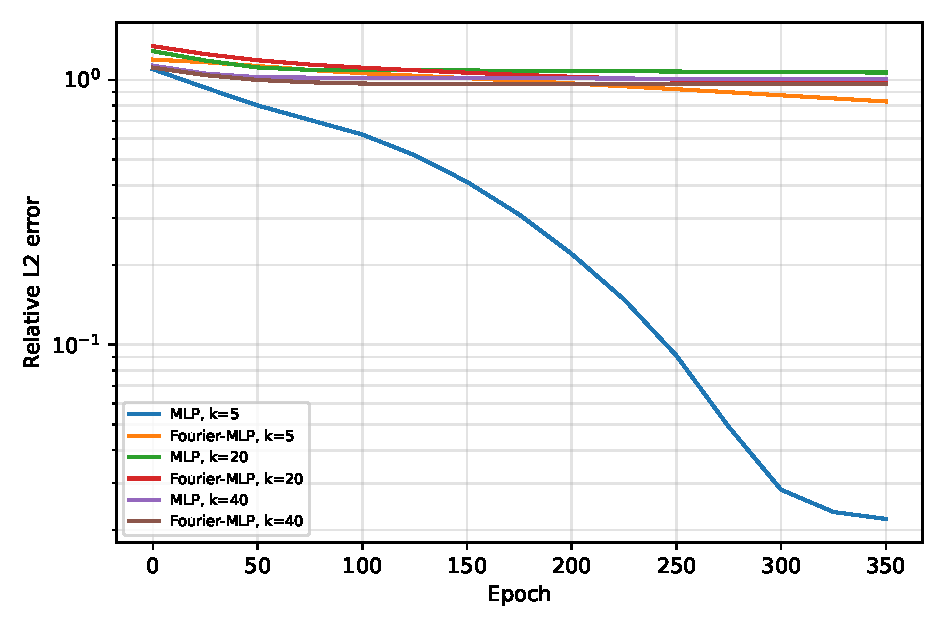
\includegraphics[width=0.78\textwidth]{figures/fig_pinn_training.pdf}
    \caption{Helmholtz-PINN 实验中的相对 $L^2$ 误差训练曲线。高波数问题明显更难训练。}
    \label{fig:pinn-training}
\end{figure}

图\ref{fig:pinn-solutions}给出了 $k=10$ 和 $k=40$ 时的最终近似解。高波数下,普通 MLP-PINN 难以捕捉正确振荡结构；Fourier-PINN 在部分波数上改善残差,但仍可能出现相位误差或振幅误差。该结果说明,对于 Helmholtz 方程,单纯更换输入特征并不足以完全克服强形式 PINN 的困难,还需要结合更合适的损失尺度、采样策略或变分结构。

\begin{figure}[H]
    \centering
    \subfigure[$k=10$]{
        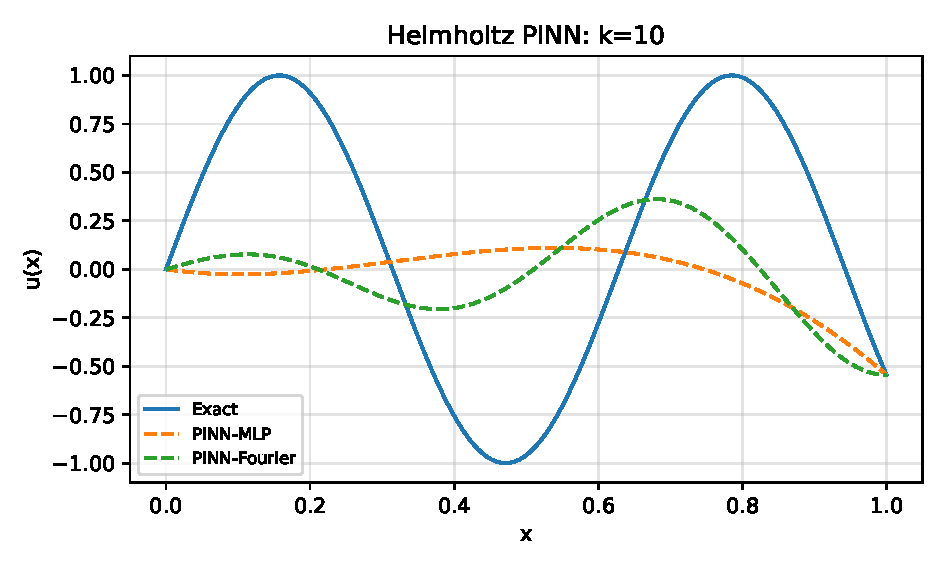
\includegraphics[width=0.48\textwidth]{figures/fig_pinn_solution_k10.pdf}
    }
    \hfill
    \subfigure[$k=40$]{
        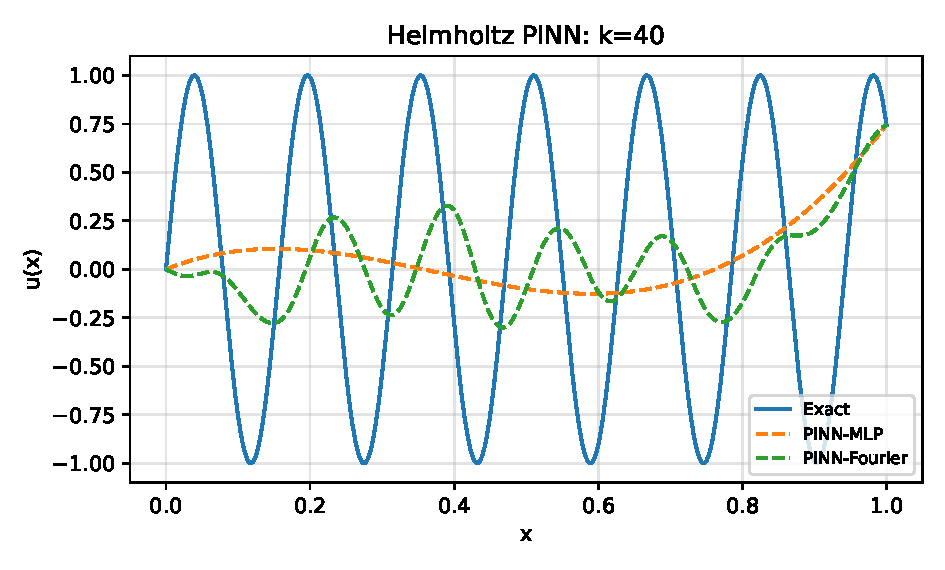
\includegraphics[width=0.48\textwidth]{figures/fig_pinn_solution_k40.pdf}
    }
    \caption{不同波数下 Helmholtz-PINN 的最终近似解。}
    \label{fig:pinn-solutions}
\end{figure}

\subsection{实验结果的数学解释}

表\ref{tab:pinn-results}中的现象可以用式\eqref{eq:residual-fourier-norm}解释。若网络主要产生低频误差,则对于 $|\xi|\ll k$,残差权重大约为 $k^4$:
\begin{equation}\label{eq:k4-weight}
    |\xi^2-k^2|^2\approx k^4.
\end{equation}
因此同样大小的低频误差在高波数问题中会造成更大的残差。另一方面,若网络学到的频率接近但不等于 $k$,即 $\xi=k+\delta$,则
\begin{equation}\label{eq:near-frequency-weight}
    |\xi^2-k^2|^2=|2k\delta+\delta^2|^2\approx 4k^2\delta^2.
\end{equation}
这说明高波数问题不仅要求网络有高频表达能力,还要求频率和相位足够准确。普通 MLP 的谱偏差会拖慢高频学习,而强形式残差又放大频率误差,二者叠加导致 Helmholtz-PINN 的困难。

\section{改进方向讨论}

\subsection{引入与波数相关的 Fourier 特征}

由于 Helmholtz 方程的振荡频率与 $k$ 直接相关,一个自然想法是在输入层显式加入 $\sin(kx)$、$\cos(kx)$ 或更丰富的三角特征。例如可以取
\begin{equation}\label{eq:k-related-features}
    \gamma_k(x)=\bigl(x,\sin(kx),\cos(kx),\sin(2kx),\cos(2kx)\bigr).
\end{equation}
这与 Trefftz 方法的思想相近:既然方程的局部解具有波动结构,就应当让近似空间尽可能包含这类结构。Fourier features 正是神经网络语境下实现这一思想的一种方式。

不过,实验也表明,Fourier features 并不是万能的。它们能改善函数表示,但 PINN 还涉及微分残差、边界约束、优化过程和采样策略。如果残差项尺度过大,或者优化器无法有效平衡不同频率成分,训练仍可能失败。

\subsection{弱形式与变分型 PINN}

强形式 PINN 需要直接计算二阶导数,这对 Helmholtz 方程尤其敏感。变分型 PINN(Variational PINN)将弱形式写入损失函数\cite{kharazmi2019variational},通过分部积分降低导数阶数,从而可能提高训练稳定性。对于方程
\begin{equation}\label{eq:weak-helmholtz-repeat}
    -u''-k^2u=f,
\end{equation}
弱形式对应
\begin{equation}\label{eq:weak-loss-basis}
    \int_0^1 u_\theta'(x)v'(x)\,\dd x-k^2\int_0^1u_\theta(x)v(x)\,\dd x
    =\int_0^1f(x)v(x)\,\dd x.
\end{equation}
若选择一组测试函数 $\{v_j\}_{j=1}^M$,可以构造变分残差损失
\begin{equation}\label{eq:vpinn-loss}
    \calJ_{\mathrm{weak}}(\theta)
    =\sum_{j=1}^M
    \left|
    \int_0^1 u_\theta'v_j'\,\dd x-k^2\int_0^1u_\theta v_j\,\dd x-
    \int_0^1fv_j\,\dd x
    \right|^2.
\end{equation}
相比强形式残差,弱形式更接近有限元方法,也更容易引入稳定性分析。

\subsection{与传统 Helmholtz 求解器和神经算子的关系}

高频 Helmholtz 问题在传统数值计算中也不是简单问题。除有限元离散误差外,线性代数层面还需要处理强不定性带来的迭代收敛困难；例如 sweeping preconditioner、源传递、极化迹和优化 Schwarz 方法都可以理解为针对 Helmholtz 结构设计的专门预条件技术\cite{gander2019class}. 这说明 Helmholtz 方程的困难并非 PINN 独有,而是由波动算子的频率结构决定。神经网络方法若要在此类问题上稳定工作,也需要吸收传统数值分析中的结构化思想,而不是仅依赖通用优化器。

另一方面,神经算子方法试图学习解算子
\begin{equation}\label{eq:operator-learning}
    \mathcal G: f\mapsto u,\qquad \calL_k u=f,
\end{equation}
而不是对每一个右端项重新训练一个网络。Fourier Neural Operator 在 Fourier 空间中参数化积分核,对具有平移不变或近似平移不变结构的问题尤其自然\cite{li2021fourier}；一般 neural operator 框架则把神经网络推广为函数空间之间的映射\cite{kovachki2023neural}。不过,对于高波数 Helmholtz 方程,算子族随 $k$ 的变化、边界条件以及共振附近的稳定性仍然是必须处理的核心问题。

\subsection{采样策略与损失尺度}

高波数问题需要足够密集的采样点。若每个波长上的采样点过少,损失函数无法分辨振荡结构。设希望每个波长至少有 $m$ 个采样点,则由式\eqref{eq:points-per-wavelength}可得
\begin{equation}\label{eq:sampling-condition}
    h_s\lesssim \frac{2\pi}{mk},
    \qquad
    N_r\gtrsim \frac{mk}{2\pi}.
\end{equation}
另一方面,Helmholtz 残差中 $k^2u$ 项随波数增大而放大,因此损失函数可能需要适当归一化,例如使用式\eqref{eq:normalized-residual}。更进一步,可以使用自适应采样,在残差较大的区域增加采样点:
\begin{equation}\label{eq:adaptive-sampling}
    \rho(x)\propto |r_\theta(x)|^p+\varepsilon,
    \qquad p>0,
\end{equation}
其中 $\rho$ 是新的采样密度,$\varepsilon$ 防止采样概率为零。

\section{结论}

本文讨论了神经网络的谱偏差及其在 Helmholtz 方程求解中的影响。谱偏差说明,标准神经网络训练通常低频优先,而高频成分收敛较慢。Helmholtz 方程在高波数下具有明显振荡结构,因而成为检验神经网络 PDE 求解能力的典型问题。

从 Fourier 分析看,Helmholtz 算子的符号为 $p_k(\xi)=\xi^2-k^2$。这意味着残差对频率非常敏感:低频误差会被约 $k^2$ 放大,而接近特征频率的微小频率偏差也会产生 $2k\delta$ 量级的残差。由此可见,Helmholtz-PINN 的困难不仅来自解的高频性,还来自强形式残差中 $-u_\theta''$ 与 $k^2u_\theta$ 的敏感抵消。采样点不足时,PINN 还可能只在离散点上降低残差,而无法保证区间内部的振荡结构正确。

实验结果支持上述判断。普通 MLP 在函数拟合中明显偏向低频目标,对高频目标误差下降缓慢；在一维 Helmholtz-PINN 中,波数增大导致误差和残差显著恶化。Fourier features 能有效改善高频函数拟合,并在高波数 PINN 中降低部分残差,但不能单独完全解决强形式 PINN 的训练困难。因此,对于 Helmholtz 方程这类振荡型 PDE,神经网络方法必须结合频率结构、采样分辨率、损失归一化和变分思想进行设计,而不能简单依赖普通 MLP 的通用逼近能力。

总体而言,谱偏差为理解神经网络求解振荡型 PDE 的局限提供了清晰解释。它提示我们:科学机器学习并不是用神经网络替代所有传统数值方法,而是要把 PDE 的数学结构、频率特征和机器学习的优化机制结合起来。对于 Helmholtz 方程,未来更有前景的方向可能是 Fourier-feature PINN、Trefftz 型神经网络、弱形式 PINN 以及神经算子方法之间的结合；其中 Fourier Neural Operator 和更一般的 neural operator 框架提供了从函数空间到函数空间学习 PDE 解算子的另一条路线\cite{li2021fourier,kovachki2023neural}.

\bibliographystyle{plain}
\bibliography{references}

\end{document}
